
\section{Laboratory Methods}
(such as data and error analysis, electronics,
instrumentation, radiation detection,
counting statistics, interaction of
charged particles with matter, lasers
and optical interferometers, dimensional
analysis, fundamental applications
of probability and statistics)

%%%%%%%%%%%%%%%%%%%%%%%%%%%%%%%%%%%%%%%

\subsection{Data and error analysis} 
\Table{
\hline

Semi-log (lin-log and log-lin) & \begin{minipage}{.375\textwidth}
      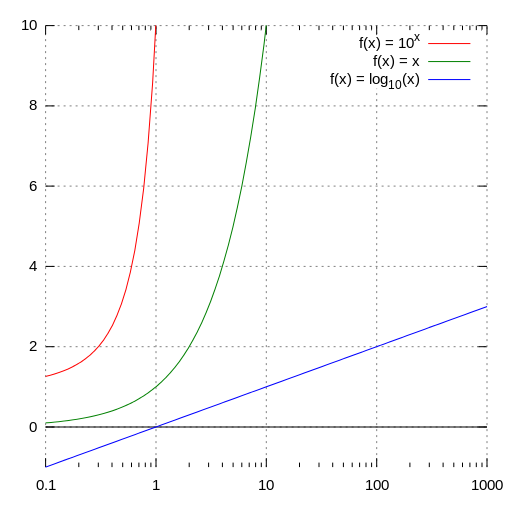
\includegraphics[width=\linewidth, height=60mm]{images/LinLog.png}
    \end{minipage} \\
    
Plot 3 characteristic $f(x)$ & \begin{minipage}{.375\textwidth}
      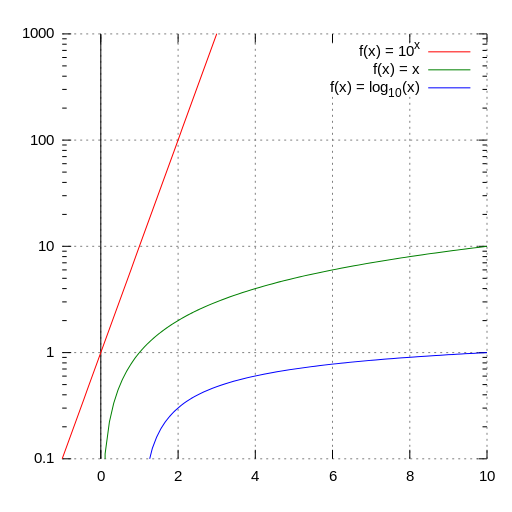
\includegraphics[width=\linewidth, height=60mm]{images/LogLin.png}
      \tiny \url{https://en.wikipedia.org/wiki/Semi-log_plot}
    \end{minipage} 

\\ \hline

Plot 3 characteristic $f(x)$ for log-log &\begin{minipage}{.375\textwidth}
      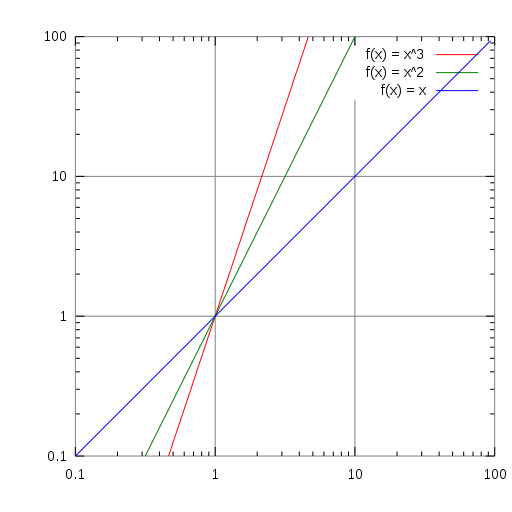
\includegraphics[width=\linewidth, height=60mm]{images/LogLog.png}
      \tiny \url{https://en.wikipedia.org/wiki/Log\%E2\%80\%93log_plot}
    \end{minipage} 
 
  \\ \hline
}


\Table{
\hline

\MiniPg{.5}{
Uncertainty or error $\delta R$ for $R(X,Y,...)$
}

&

\MiniPg{.5}{\center
$\delta R = \sqrt{ \Big(\dfrac{\partial R}{\partial X} \cdot \delta X \Big)^2 + \Big( \dfrac{\partial R}{\partial Y } \cdot \delta Y \Big)^2 + ... }$
}

\\ \hline
\MiniPg{.5}{
Addition of measured quantities
}

&

\MiniPg{.5}{
\center
$R = X + Y -Z$


$\delta R \approx \delta X + \delta Y + \delta Z$

$\delta R = \sqrt{(\delta X)^2 + (\delta Y)^2 + (\delta Z)^2} $

}

\\ \hline
\MiniPg{.5}{
Multiplication of measured quantities
}

&

\MiniPg{.5}{
\center
$R = \dfrac{X \cdot Y}{ Z}$


$\dfrac{\delta R}{|R|} \approx \dfrac{\delta X}{|X|} + \dfrac{\delta Y}{|Y|} + \dfrac{\delta Z}{|Z|}$

$\delta R = |R| \cdot \sqrt{\Big(\dfrac{\delta X}{|X|}\Big)^2 + \Big(\dfrac{\delta Y}{|Y|}\Big)^2 +\Big (\dfrac{\delta Z}{|Z|}\Big)^2} $

}

\\ \hline
\MiniPg{.5}{
Multiplication of with a constant
}

&

\MiniPg{.5}{
\center
$R = c \cdot X$

$\delta R = |c| \cdot \delta X $

}

\\ \hline
\MiniPg{.5}{
Polynomial functions
}

&

\MiniPg{.5}{
\center
$R = X^n$

$\delta R = |R| \cdot |n| \cdot \dfrac{\delta X}{|X|}  $

\tiny \url{http://lectureonline.cl.msu.edu/~mmp/labs/error/e2.htm}

}

\\ \hline
}


%%%%%%%%%%%%%%%%%%%%%%%%%%%%%%%%%%%%%%%

\subsection{Electronics} 

%%%%%%%%%%%%%%%%%%%%%%%%%%%%%%%%%

\subsection{Instrumentation} 

%%%%%%%%%%%%%%%%%%%%%%%%%%%%%%%%%

\subsection{Radiation detection} 

%%%%%%%%%%%%%%%%%%%%%%%%%%%%%%%%%

\subsection{Counting statistics} 
\center
\begin{tabular}{|c|c|}
\hline

Poisson distribution &  $P(k \textrm{ events in interval}) = \dfrac{\lambda^ke^{-k}}{k!}$ \\
\hline
When to use? & $\lambda$ is the avg. \# of events per interval. \\
& $k$ is the integer \# of times an event occurs in an interval. \\
& Events occur independently. \\
& Constant rate of occurrence. \\
& Events cannot be identical in space and time. \\
& Probability of an event in an interval $\propto$ length of interval. \\
& e.g. \# of decays from a radioactive sample over 1 hour. \\
\hline
Properties & mean = variance = $\lambda$, so $\sigma = \sqrt{\textrm{var}} = \sqrt{\lambda}$ \\
& If $\lambda > $ about 10, normal distribution is good approximation \\
& if continuity correction is used. See:\\
& \url{https://en.wikipedia.org/wiki/Poisson_distribution}

 \\ \hline
\end{tabular}
\flushleft

\subsection{Interaction of charged particles with matter} 

%%%%%%%%%%%%%%%%%%%%%%%%%%%%%%%%%

\subsection{Lasers and optical interferometers} 

\Table{
\hline

Laser

&

\MiniPg{.7}{
\center
Light amplification by stimulated emission of radiation

\GraphicWHN{.75}{.5}{laser.jpg}
\tiny \url{http://micro.magnet.fsu.edu/primer/java/lasers/stimulatedemission/}

}

\\ \hline
}

%%%%

\Table{
\hline

Stimulated emission

&
\MiniPg{.7}{
\GraphicWHN{.8}{.4}{stimulatedEmission.png}
\tiny \url{https://en.wikipedia.org/wiki/Laser}
}
\\ \hline
}


%%%%%%%%%%%%%%%%%%%%%%%%%%%%%%%%%

\subsection{Dimensional analysis} 

%%%%%%%%%%%%%%%%%%%%%%%%%%%%%%%%%

\subsection{Fundamental applications of probability and statistics}  


